\section{Pilot Application: NDNEX}

\subsection{Introduction}

Our pilot application for this network environment is \textbf{NDNEx} (NDN-Exercise) and related a user-facing \textbf{Identity Manager}.  Supporting physical activity is both a critical part of building healthy communities and a key retail market. Per the original proposal, we focus on a consumer-facing application, as shown in Figure~\ref{fig:continuum}, rather than clinical applications or other with formal connections to the healthcare system. 

NDNEx is a mobile physical activity monitoring application (fitness tracker) that supports location-based notifications / content push. Commercial parallels include  Nike+, Fitbit, Endomondo (see Figure~\ref{fig:endomondo}), etc. It also is a non-proprietary ecosystem for consumer physical activity data. Following the philosophy of Open mHealth, our objective is to create NDNEx, which is perceived by the user as a single application, through  a \textbf{simple ecosystem of composable services} rather than siloed application. In this way, it is to act as an example of interoperating components of an Open mHealth ecosystem.  This places additional requirements on the design. 

NDNEx targets  the following features for the end-user:
\begin{itemize}
\item Capture and report walking, jogging, and running activity. 
\item Calculate and report activity metrics based on GPS and accelerometer data for both automatically and self-identified rounds of exercise.  
\item Support comparison within ad-hoc and formal groups or teams. 
\item Provide location-based content push during the exercise, which can be used for health, entertainment, local, and team-related content. 
\end{itemize}

The Open mHealth team envisions that the Internet will interconnect 1)
data capture, 2) secure storage, 3) modeling and analytics, and 4) user
interface components to create a modular, layered sense-making framework.
NDNEx will include examples of each of these pieces, which are described in
more detail in the next section.

\begin{figure*}
\begin{center}
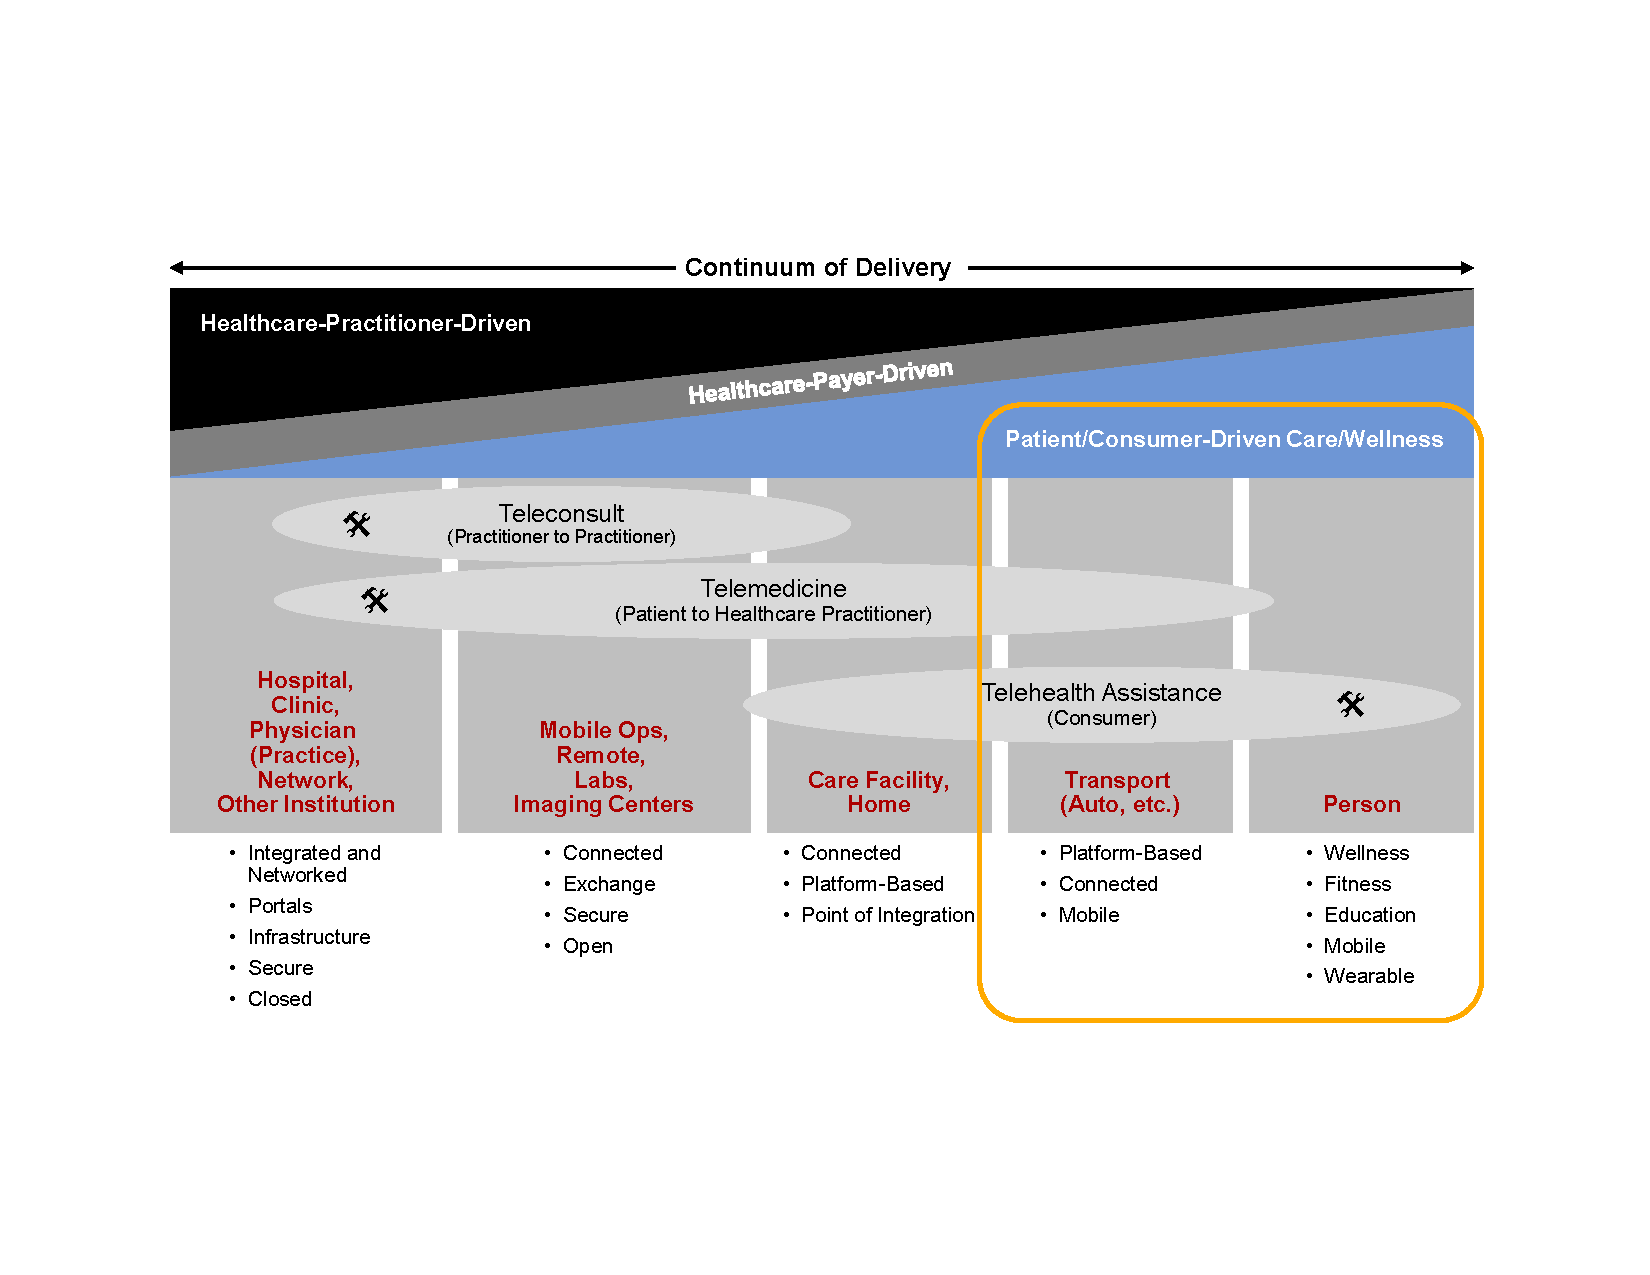
\includegraphics[width=.8\textwidth]{figures/continuum}
\caption{{Focus of Open mHealth network environment shown in yellow box. Figure from Gartner, 2013.  }}
% A Framework for Understanding Telehealth, Telemedicine and Other Remote Healthcare Delivery Solutions
% need to redraw before release
\label{fig:continuum}
\end{center}
\end{figure*}

\begin{figure}
\begin{center}
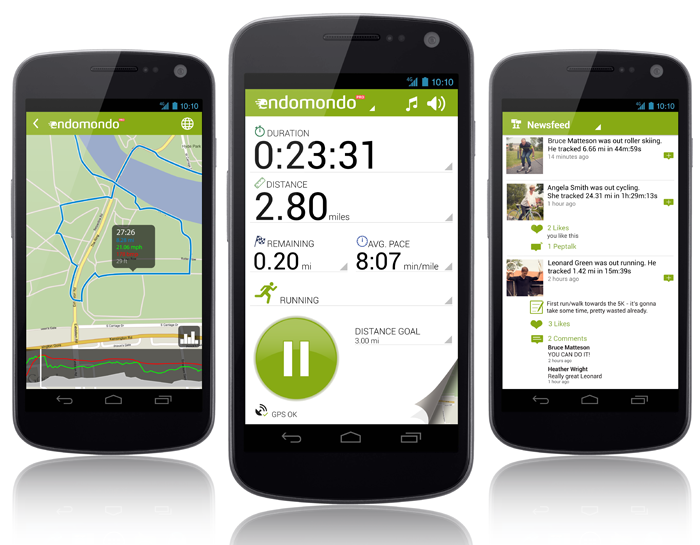
\includegraphics[width=.6\textwidth]{figures/endomondo}
\caption{Endomondo commercial fitness tracker. \protect\url{https://www.endomondo.com/}}
\label{fig:endomondo}
\end{center}
\end{figure}

\begin{figure}
\begin{center}
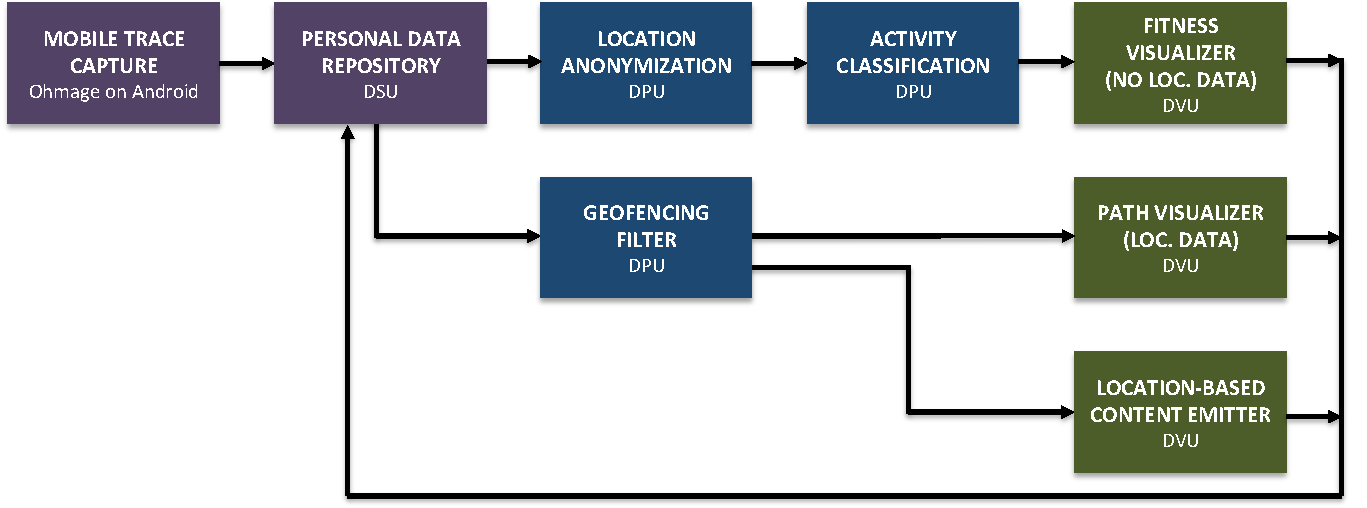
\includegraphics[width=1\textwidth]{figures/ConceptualBlock}
\caption{Conceptual block diagram showing data flow.}
\label{fig:ConceptualBlock}
\end{center}
\end{figure}

NDNEx requires specific design of the following, as an example of the Open mHealth network environment.  
\begin{itemize}
\item Namespace / schema 
\item Repository / storage 
\item Service composability
\item Authentication / identity assurance
\item Data provenance
\item Access auditing
\item Mobile publishing
\item Legal requirements for success
\end{itemize}

\subsection{Application Requirements}

Fundamentally, NDNEx is to be achieved through an open-data ecosystem that follows the Open mHealth paradigm, but adapting its REST-based communication model to a data dissemination approach using NDN.  Each component could be provided by  different service providers at different stages in the processing chain, rather than a siloed application.

The design should rely as much as possible on basic NDN primitives (hierarchical naming, interest/data exchange, sync, repositories, keys-as-data, etc.) as possible, rather than designing new protocols.    Given that Open mHealth already envisions a data-centric thin waist in their ecosystem, NDN provides much more relevant functionality at the network layer than IP.   So basic solutions in NDN have much more direct impact on the scalability, security, and ease of development; we need not build up additional layers on IP to get near the app challenges.

The application architecture should be consistent with the pieces above and from previous participatory sensing projects. (e.g., Mun et al, 2009)
  
%% Repeated from above.
\subsubsection{Naming} 
\begin{itemize}
\item \textbf{Data format namespace design} shall come directly from Open mHealth developer documentation. 
\item \textbf{Name and data} schemes should direct mappings of Open mHealth schema
\item Borrow ideas from Named Function Networking concept for distributed processing
\item Consumers should be able to access raw and processed data for a certain time period.
\item Consumers should be able to efficiently read data sequentially. 
\item Data will include:
    \begin{itemize}
    \item Raw time-location data (GPS, accelerometer) from mobiles. 
    \item Successive rounds of processing that, for example:  
        \begin{itemize}
        \item Generate classified activity data that follows the Physical Activity JSON schema and perhaps other related schemas.  (This happens at client-side in Ohmage Mobility but could happen at a DPU.)	
        \item Identify / segment ``bouts”''of physical activity or exercise. 
        \item Add features to a bout from DPUs to the existing store. 
        \end{itemize}
    \end{itemize}
    \item End-user configuration information
    \item Identity and trust related data
\end{itemize} 

\subsubsection{Trust and security}

Our objective is to see how well the NDN architectural mechanisms fit into security requirements, and propose new ones where necessary. 
\begin{itemize}
\item \textbf{Identity and trust management} scenario shall come from the notion of NDNEx as consisting of interoperating components in an ecosystem, not a silo'd application. 
\item All data should be encrypted
\item Provide granular access control over various components of the data namespace – in particular, raw location data.  
\item Doing better than Oauth2 for securing distributed processing is critical
\item Follow passive key publication approach (rather than active) if possible. 
\item If possible, we should support different identities relative each part of the system: collection, processing, and visualization, such as:
    \begin{itemize}
    \item Collection: User may publish data to serve multiple applications, but doesn’t want them to be able to conspire / correlate that they are the same user.
    \item Processing:  Design should provide the minimum possible information to the processing components about user identity. 
    \item Visualization: Visible face of “the app” to the user. 
    \end{itemize}
\end{itemize}

\subsubsection{Storage in the network}
\begin{itemize}
\item Each user may choose a different storage provider, though we may only have one option in the initial implementation
\item Interaction of personal and shared stores
\item New legal / economic relationship between the players
\end{itemize}
